\subsection*{attention\_block on the Mac (M4 Pro, 8 threads): verdict \emph{interaction}}
The slow state differs from the fast state in 63 switches. Fast 0.919~ms vs.\ slow 1.250~ms (+36.1\%); $\tau$ = 0.017~ms. ddmin needed 16 judge evaluations (versus 63 for leave-one-out, 1953 for all pairs) and returned the culprit set \code{-joint/joint\_\allowbreak{}graph.\allowbreak{}patterns/\_\allowbreak{}sfdp\_\allowbreak{}pattern\_\allowbreak{}11\_\allowbreak{}inference}, \code{-joint/joint\_\allowbreak{}graph.\allowbreak{}patterns/\_\allowbreak{}sfdp\_\allowbreak{}pattern\_\allowbreak{}12\_\allowbreak{}inference}. Each culprit alone was judged \emph{fast}: the slowdown needs all of them together. \textbf{Kernel-level explanation.} fused kernels 1 $\rightarrow$ 4, extern calls 3 $\rightarrow$ 4, intermediate bytes 4,198,400 $\rightarrow$ 11,591,680. Kernels gained: \code{cpp\_\allowbreak{}fused\_\allowbreak{}\_\allowbreak{}softmax\_\allowbreak{}abs\_\allowbreak{}all\_\allowbreak{}amax\_\allowbreak{}div\_\allowbreak{}eq\_\allowbreak{}mul\_\allowbreak{}ne\_\allowbreak{}sub\_\allowbreak{}view}, \code{cpp\_\allowbreak{}fused\_\allowbreak{}clone\_\allowbreak{}split\_\allowbreak{}transpose\_\allowbreak{}view}, \code{cpp\_\allowbreak{}fused\_\allowbreak{}clone\_\allowbreak{}transpose\_\allowbreak{}view}. Extern calls lost: \code{torch.\allowbreak{}ops.\allowbreak{}aten.\allowbreak{}\_\allowbreak{}scaled\_\allowbreak{}dot\_\allowbreak{}product\_\allowbreak{}flash\_\allowbreak{}attention\_\allowbreak{}for\_\allowbreak{}cpu}; gained: \code{extern\_\allowbreak{}kernels.\allowbreak{}bmm} ($\times$2). Rules suppressed in the culprit state: \code{\_\allowbreak{}sfdp\_\allowbreak{}pattern\_\allowbreak{}11\_\allowbreak{}inference}, \code{\_\allowbreak{}sfdp\_\allowbreak{}pattern\_\allowbreak{}12\_\allowbreak{}inference}. 
\begin{table}[h]\centering\small
\begin{tabular}{lp{0.62\linewidth}}\toprule
field & value \\\midrule
\textbf{model} & attention\_block (Chideras-MacBook-Pro-2) \\
judge & timing (median\_ms) \\
fast reference & 0.926 ms, $\tau$ = 0.017 ms (1.8\%) \\
slow state & 1.250 ms \\
candidate changes & 63 \\
judge evaluations & 16 \\
verdict & interaction \\
culprits & \code{\_\allowbreak{}sfdp\_\allowbreak{}pattern\_\allowbreak{}11\_\allowbreak{}inference}, \code{\_\allowbreak{}sfdp\_\allowbreak{}pattern\_\allowbreak{}12\_\allowbreak{}inference} \\
kernels fast $\rightarrow$ culprits & 1 $\rightarrow$ 4 \\
extern calls & 3 $\rightarrow$ 4 \\
intermediate bytes & 4,198,400 $\rightarrow$ 11,591,680 \\
median ms & 0.919 $\rightarrow$ 1.244 \\
\bottomrule\end{tabular}
\caption{Attribution summary, attention\_block.}
\end{table}
\IfFileExists{figures/trace_attention_block_mac.pdf}{\begin{figure}[h]\centering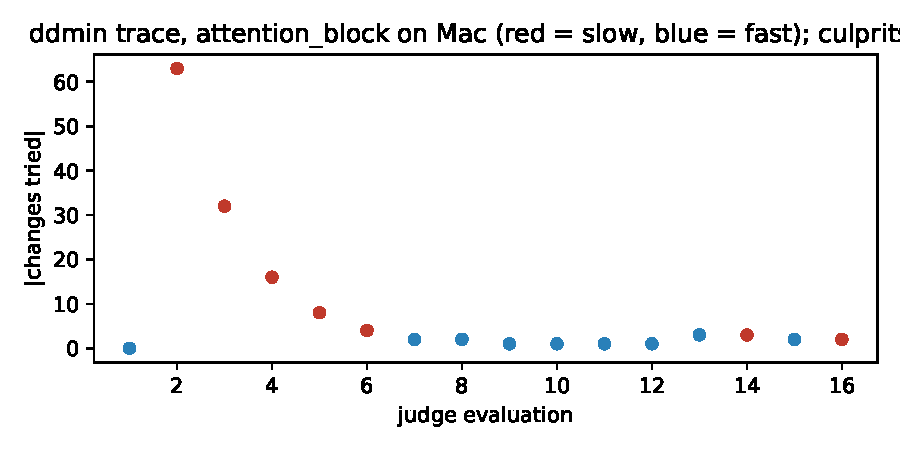
\includegraphics[width=0.7\linewidth]{figures/trace_attention_block_mac.pdf}\caption{ddmin search trace for attention\_block (Mac (M4 Pro, 8 threads)): each point is one judge evaluation.}\end{figure}}{}

\subsection*{decode\_mlp on the Mac (M4 Pro, 8 threads): verdict \emph{single}}
The slow state differs from the fast state in 16 switches. Fast 0.195~ms vs.\ slow 0.222~ms (+14.1\%); $\tau$ = 0.011~ms. ddmin needed 7 judge evaluations (versus 16 for leave-one-out, 120 for all pairs) and returned the culprit set \code{+optimus/decompose\_\allowbreak{}mm\_\allowbreak{}pass}. A single change reproduces the whole slowdown. \textbf{Kernel-level explanation.} fused kernels 1 $\rightarrow$ 1, extern calls 3 $\rightarrow$ 0, intermediate bytes 20,480 $\rightarrow$ 20,480. Kernels lost: \code{cpp\_\allowbreak{}fused\_\allowbreak{}mul\_\allowbreak{}silu}. Kernels gained: \code{cpp\_\allowbreak{}fused\_\allowbreak{}mm\_\allowbreak{}mul\_\allowbreak{}silu\_\allowbreak{}t}. Extern calls lost: \code{extern\_\allowbreak{}kernels.\allowbreak{}mm} ($\times$3); gained: none. 
\begin{table}[h]\centering\small
\begin{tabular}{lp{0.62\linewidth}}\toprule
field & value \\\midrule
\textbf{model} & decode\_mlp (Chideras-MacBook-Pro-2) \\
judge & timing (median\_ms) \\
fast reference & 0.194 ms, $\tau$ = 0.011 ms (5.5\%) \\
slow state & 0.222 ms \\
candidate changes & 16 \\
judge evaluations & 7 \\
verdict & single \\
culprits & \code{+optimus/decompose\_\allowbreak{}mm\_\allowbreak{}pass} \\
kernels fast $\rightarrow$ culprits & 1 $\rightarrow$ 1 \\
extern calls & 3 $\rightarrow$ 0 \\
intermediate bytes & 20,480 $\rightarrow$ 20,480 \\
median ms & 0.195 $\rightarrow$ 0.223 \\
\bottomrule\end{tabular}
\caption{Attribution summary, decode\_mlp.}
\end{table}
\IfFileExists{figures/trace_decode_mlp_mac.pdf}{\begin{figure}[h]\centering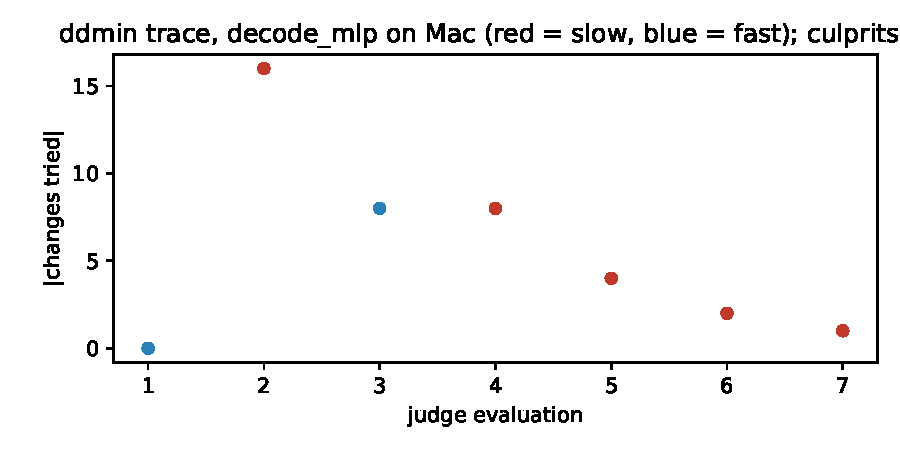
\includegraphics[width=0.7\linewidth]{figures/trace_decode_mlp_mac.pdf}\caption{ddmin search trace for decode\_mlp (Mac (M4 Pro, 8 threads)): each point is one judge evaluation.}\end{figure}}{}

\subsection*{norm\_mlp on the Mac (M4 Pro, 8 threads): verdict \emph{single}}
The slow state differs from the fast state in 8 switches. Fast 1.061~ms vs.\ slow 1.099~ms (+3.6\%); $\tau$ = 0.018~ms. ddmin needed 8 judge evaluations (versus 8 for leave-one-out, 28 for all pairs) and returned the culprit set \code{-joint/constant\_\allowbreak{}folding}. A single change reproduces the whole slowdown. \textbf{Kernel-level explanation.} fused kernels 3 $\rightarrow$ 3, extern calls 2 $\rightarrow$ 2, intermediate bytes 1,573,376 $\rightarrow$ 1,573,376. Kernels lost: \code{cpp\_\allowbreak{}fused\_\allowbreak{}add\_\allowbreak{}gelu\_\allowbreak{}mean\_\allowbreak{}mul\_\allowbreak{}pow}. Kernels gained: \code{cpp\_\allowbreak{}fused\_\allowbreak{}add\_\allowbreak{}gelu\_\allowbreak{}mean\_\allowbreak{}mul\_\allowbreak{}pow\_\allowbreak{}reciprocal}. 
\begin{table}[h]\centering\small
\begin{tabular}{lp{0.62\linewidth}}\toprule
field & value \\\midrule
\textbf{model} & norm\_mlp (Chideras-MacBook-Pro-2) \\
judge & timing (median\_ms) \\
fast reference & 1.058 ms, $\tau$ = 0.018 ms (1.7\%) \\
slow state & 1.099 ms \\
candidate changes & 8 \\
judge evaluations & 8 \\
verdict & single \\
culprits & \code{-joint/constant\_\allowbreak{}folding} \\
kernels fast $\rightarrow$ culprits & 3 $\rightarrow$ 3 \\
extern calls & 2 $\rightarrow$ 2 \\
intermediate bytes & 1,573,376 $\rightarrow$ 1,573,376 \\
median ms & 1.061 $\rightarrow$ 1.085 \\
\bottomrule\end{tabular}
\caption{Attribution summary, norm\_mlp.}
\end{table}
\IfFileExists{figures/trace_norm_mlp_mac.pdf}{\begin{figure}[h]\centering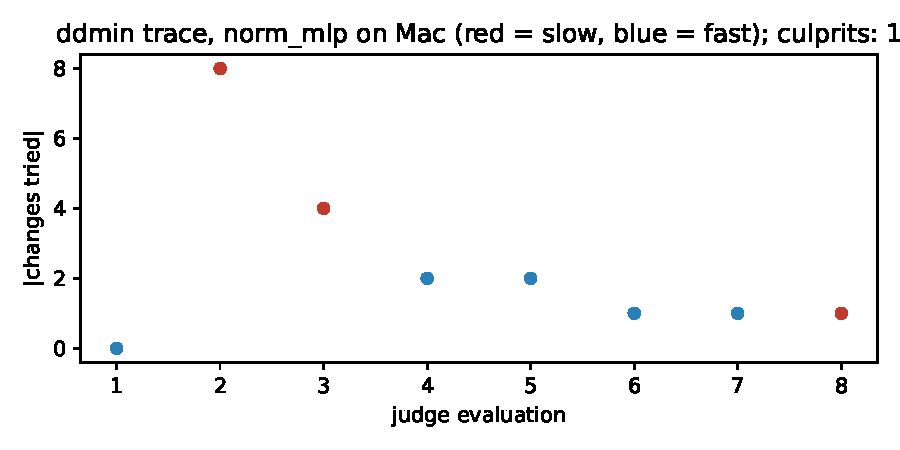
\includegraphics[width=0.7\linewidth]{figures/trace_norm_mlp_mac.pdf}\caption{ddmin search trace for norm\_mlp (Mac (M4 Pro, 8 threads)): each point is one judge evaluation.}\end{figure}}{}

\subsection*{resnet18 on the Mac (M4 Pro, 8 threads): verdict \emph{single}}
The slow state differs from the fast state in 6 switches. Fast 26.205~ms vs.\ slow 29.119~ms (+11.1\%); $\tau$ = 0.576~ms. ddmin needed 5 judge evaluations (versus 6 for leave-one-out, 15 for all pairs) and returned the culprit set \code{-lowering/layout\_\allowbreak{}optimization}. A single change reproduces the whole slowdown. \textbf{Kernel-level explanation.} fused kernels 14 $\rightarrow$ 12, extern calls 21 $\rightarrow$ 21, intermediate bytes 30,052,352 $\rightarrow$ 6,470,912. Kernels lost: \code{cpp\_\allowbreak{}fused\_\allowbreak{}\_\allowbreak{}native\_\allowbreak{}batch\_\allowbreak{}norm\_\allowbreak{}legit\_\allowbreak{}no\_\allowbreak{}training\_\allowbreak{}add\_\allowbreak{}convolution\_\allowbreak{}relu} ($\times$7), \code{cpp\_\allowbreak{}fused\_\allowbreak{}\_\allowbreak{}native\_\allowbreak{}batch\_\allowbreak{}norm\_\allowbreak{}legit\_\allowbreak{}no\_\allowbreak{}training\_\allowbreak{}convolution\_\allowbreak{}max\_\allowbreak{}pool2d\_\allowbreak{}with\_\allowbreak{}indices\_\allowbreak{}relu}, \code{cpp\_\allowbreak{}fused\_\allowbreak{}convolution}. Kernels gained: \code{cpp\_\allowbreak{}fused\_\allowbreak{}\_\allowbreak{}native\_\allowbreak{}batch\_\allowbreak{}norm\_\allowbreak{}legit\_\allowbreak{}no\_\allowbreak{}training\_\allowbreak{}add\_\allowbreak{}relu} ($\times$6), \code{cpp\_\allowbreak{}fused\_\allowbreak{}\_\allowbreak{}native\_\allowbreak{}batch\_\allowbreak{}norm\_\allowbreak{}legit\_\allowbreak{}no\_\allowbreak{}training\_\allowbreak{}max\_\allowbreak{}pool2d\_\allowbreak{}with\_\allowbreak{}indices\_\allowbreak{}relu}. 
\begin{table}[h]\centering\small
\begin{tabular}{lp{0.62\linewidth}}\toprule
field & value \\\midrule
\textbf{model} & resnet18 (Chideras-MacBook-Pro-2) \\
judge & timing (median\_ms) \\
fast reference & 26.118 ms, $\tau$ = 0.576 ms (2.2\%) \\
slow state & 29.119 ms \\
candidate changes & 6 \\
judge evaluations & 5 \\
verdict & single \\
culprits & \code{-lowering/layout\_\allowbreak{}optimization} \\
kernels fast $\rightarrow$ culprits & 14 $\rightarrow$ 12 \\
extern calls & 21 $\rightarrow$ 21 \\
intermediate bytes & 30,052,352 $\rightarrow$ 6,470,912 \\
median ms & 26.205 $\rightarrow$ 29.007 \\
\bottomrule\end{tabular}
\caption{Attribution summary, resnet18.}
\end{table}
\IfFileExists{figures/trace_resnet18_mac.pdf}{\begin{figure}[h]\centering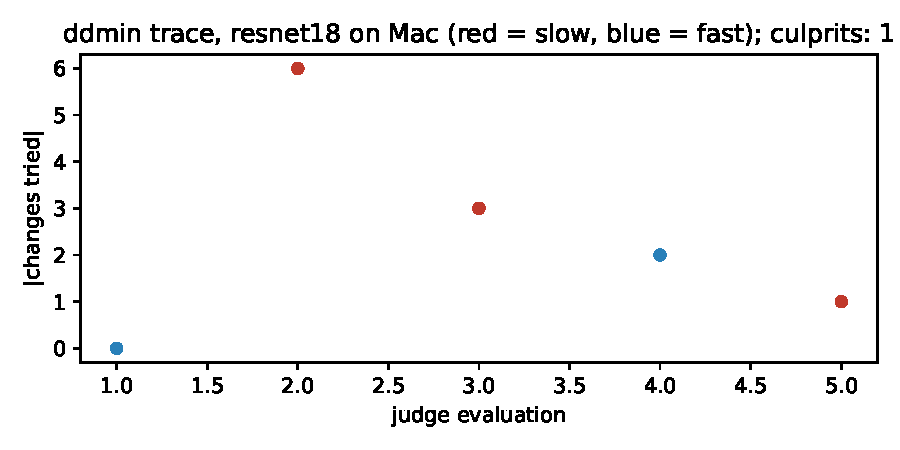
\includegraphics[width=0.7\linewidth]{figures/trace_resnet18_mac.pdf}\caption{ddmin search trace for resnet18 (Mac (M4 Pro, 8 threads)): each point is one judge evaluation.}\end{figure}}{}

\subsection*{attention\_block on the VM (Xeon, 4 threads): verdict \emph{single}}
The slow state differs from the fast state in 63 switches. Fast 7.621~ms vs.\ slow 8.265~ms (+8.4\%); $\tau$ = 0.162~ms. ddmin needed 8 judge evaluations (versus 63 for leave-one-out, 1953 for all pairs) and returned the culprit set \code{+joint/joint\_\allowbreak{}graph.\allowbreak{}patterns/\_\allowbreak{}sfdp\_\allowbreak{}pattern\_\allowbreak{}11\_\allowbreak{}inference}. A single change reproduces the whole slowdown. \textbf{Kernel-level explanation.} fused kernels 4 $\rightarrow$ 1, extern calls 4 $\rightarrow$ 3, intermediate bytes 11,591,680 $\rightarrow$ 4,198,400. Kernels lost: \code{cpp\_\allowbreak{}fused\_\allowbreak{}\_\allowbreak{}softmax\_\allowbreak{}abs\_\allowbreak{}all\_\allowbreak{}amax\_\allowbreak{}div\_\allowbreak{}eq\_\allowbreak{}mul\_\allowbreak{}ne\_\allowbreak{}sub\_\allowbreak{}view}, \code{cpp\_\allowbreak{}fused\_\allowbreak{}clone\_\allowbreak{}split\_\allowbreak{}transpose\_\allowbreak{}view}, \code{cpp\_\allowbreak{}fused\_\allowbreak{}clone\_\allowbreak{}transpose\_\allowbreak{}view}. Extern calls lost: \code{extern\_\allowbreak{}kernels.\allowbreak{}bmm} ($\times$2); gained: \code{torch.\allowbreak{}ops.\allowbreak{}aten.\allowbreak{}\_\allowbreak{}scaled\_\allowbreak{}dot\_\allowbreak{}product\_\allowbreak{}flash\_\allowbreak{}attention\_\allowbreak{}for\_\allowbreak{}cpu}. 
\begin{table}[h]\centering\small
\begin{tabular}{lp{0.62\linewidth}}\toprule
field & value \\\midrule
\textbf{model} & attention\_block (fa26-cs598a-010) \\
judge & timing (median\_ms) \\
fast reference & 7.650 ms, $\tau$ = 0.162 ms (2.1\%) \\
slow state & 8.265 ms \\
candidate changes & 63 \\
judge evaluations & 8 \\
verdict & single \\
culprits & \code{\_\allowbreak{}sfdp\_\allowbreak{}pattern\_\allowbreak{}11\_\allowbreak{}inference} \\
kernels fast $\rightarrow$ culprits & 4 $\rightarrow$ 1 \\
extern calls & 4 $\rightarrow$ 3 \\
intermediate bytes & 11,591,680 $\rightarrow$ 4,198,400 \\
median ms & 7.621 $\rightarrow$ 8.326 \\
\bottomrule\end{tabular}
\caption{Attribution summary, attention\_block.}
\end{table}
\IfFileExists{figures/trace_attention_block_vm.pdf}{\begin{figure}[h]\centering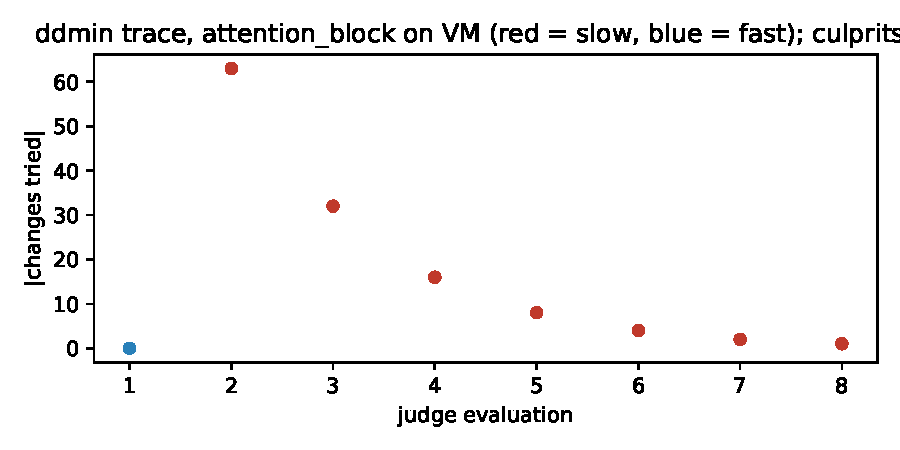
\includegraphics[width=0.7\linewidth]{figures/trace_attention_block_vm.pdf}\caption{ddmin search trace for attention\_block (VM (Xeon, 4 threads)): each point is one judge evaluation.}\end{figure}}{}%
